\chapter{Aportes}

%objetivo 1: integracion de fof + herramientas.

\section{Extendiendo Heterogenius con Herramientas de L'ogica de Primer Orden}

Existen numerosas herramientas que funcionan con el lenguaje de l'ogica de primer orden \textit{TPTP-FOF}. Para permitir la integraci'on de estas herramientas con Heterogenius y abrir el camino para la interacci'on con las futuras tecnologias basadas en 'este lenguaje, se agreg'o \textit{TPTP-FOF} al motor de Heterogenius como un lenguaje de an'alisis.

Junto a la integraci'on de \textit{TPTP-FOF}, se incorporaron los siguientes mecanismos para poder usar las herramientas correspondientes:

\begin{itemize}
\item Se permiti'o la carga de especificaciones escritas puramente en \textit{TPTP-FOF} mediante la adaptaci'on del \textit{TPTP-Parser} [TODO: citar a Andrei Tchaltsev <tchaltsev AT itc.it>
and Alexandre Riazanov <alexandre.riazanov AT gmail.com>.]

\item Se agreg'o una $\rho-$translation desde las formulas \textit{PDOCFA} a \textit{TPTP-FOF}. [TODO: referenciar la seccion que explica esto en detalle].

\end{itemize}

Teniendo el soporte de \textit{TPTP-FOF} por parte del motor de c'alculo de secuentes de Heterogenius, integramos algunas de las herramientas mas difundidas en el 'ambito de demostradores autom'aticos de teoremas para el lenguaje \textit{TPTP-FOF}: \textit{E-Prover} y \textit{SPASS} como calculadores de secuentes; \textit{E-Prover} y \textit{Mace4} como buscadores de contraejemplos.

\subsection{Herramientas Usadas}
//TODO: revisar todo esto y explicar con mas detalle:
\subsubsection{E-Prover}

Es un demostrador autom'atico de teoremas de l'ogica de primer orden basado en el calculo por superposici'on. Adem'as realiza b'usquedas de modelos por lo cual tambi'en se usa como un buscador de contraejemplos.

\subsubsection{SPASS}

Es un demostrador autom'atico de teoremas de l'ogica de primer orden con igualdad desarrollado por el Instituto Max Planck.

Desde el 2000, tanto \textit{SPASS} como \textit{E-Prover} ocupan los primeros lugares en la competencia anual de demostradores de teoremas \textit{CASC} (CADE ATP System Competition).

\subsubsection{Mace4}

Es un buscador de modelos finitos y contraejemplos para l'ogica de primer orden.

\subsection{C'alculo de secuentes}

TODO: ver como escribir bien esta parte:

Sea $\Sigma$ la especificaci'on y

\begin{prooftree}
\AxiomC{$\alpha_1$,$\ldots$,$\alpha_n$}
\UnaryInfC{$\beta_1$,$\ldots$,$\beta_m$}
\end{prooftree}

el secuente que se quiere analizar.

Se arma una nueva f'ormula $\varphi: \bigwedge\limits_{i=1}^n{\alpha_i} \Rightarrow \bigvee\limits_{j=1}^m{ \beta_{j}}$.

Se aplica un demostrador autom'atico para ver si $\Sigma \vdash \varphi$.

Dos reglas de calculo:

\begin{prooftree}
\AxiomC{$\Sigma \vdash \varphi$}
\RightLabel{(si vale)}
\UnaryInfC{$true$}
\end{prooftree}

\begin{prooftree}
\AxiomC{$\Sigma \nvdash \varphi$}
\RightLabel{(si no vale)}
\UnaryInfC{$false$}
\end{prooftree}

TODO: otra posibilidad es que tire timeout. Hay que tener una regla para esto???

\subsection{B'usqueda de contraejemplos}

Tanto \textit{Mace4} como \textit{E-Prover} se usan para buscar contraejemplos de los secuentes \textit{TPTP-FOF}. Como las dos herramientas son buscadores de modelos, lo que se hace es armar una teoria tomando en cuenta la especificaci'on y el secuente que se quiere analizar.

Sea $\Sigma$ la especificaci'on y

\begin{prooftree}
\AxiomC{$\alpha_1$,$\ldots$,$\alpha_n$}
\UnaryInfC{$\beta_1$,$\ldots$,$\beta_m$}
\end{prooftree}

el secuente que se quiere analizar.

Se arma una nueva teor'ia $\Gamma$ tal que:

\begin{itemize}

\item $\varphi \in \Gamma$ si $\varphi \in \Sigma$.

\item $\gamma \in \Gamma$ \\
	con $\gamma: \bigwedge\limits_{i=1}^n{\alpha_i} \wedge \bigwedge\limits_{j=1}^m{\neg \beta_{j}}$

\end{itemize}

Luego se realiza una b'usqueda de un modelo para la teor'ia construida $\Gamma$. En caso de encontrar un modelo que satisfaga la teor'ia $\Gamma$ se termina la busqueda y se reporta que existe por lo menos un contraejemplo para el secuente procesado.


\subsection{Integraci'on con Heterogenius}

TODO: explicar la arq.
TODO: agregar algun diagrama.


%objetivo 2
\section{Heterogeneidad Completa}
\label{sec:heterogeneidad-verdadera}

Para ampliar las capacidades de Heterogenius extendimos el concepto de heterogeneidad para lograr tener demostraciones completamente heterog'eneas en lugar de demostraciones heterogéneas pero con secuentes homogéneos. 

La diferencia principal radica en que, con la nueva implementaci'on, los secuentes pueden soportar f'ormulas de diferentes lenguajes. As'i un secuente puede ser de tipo homogéneo o heterogéneo. En el primer caso todas las f'ormulas del secuente usan el mismo lenguaje; en el segundo las f'ormulas son de lenguajes distintos.

La ventaja de los secuentes heterogéneos es que se pueden combinar f'ormulas (lemmas, axiomas) provenientes de distintas especificaciones escritas en lenguajes diferentes. De esta forma nos podemos abstraer del lenguaje en el que están escritas y concentrarnos en el an'alisis.

La principal limitaci'on de los secuentes heterogéneos es que las herramientas (calculadores de secuentes, buscadores de contraejemplos, demostradores autom'aticos) trabajan con secuentes escritos en un solo lenguaje, o sea secuentes homogéneos. Debido a esto se proveen nuevas operaciones para el manejo de f'ormulas dentro de un secuente.

\subsection{Operaciones para el manejo de f'ormulas}

Cada una de las siguientes operaciones puede cambiar o no la heterogeneidad de un secuente.  Dependiendo de los lenguajes de las f'ormulas del resultado, el secuente puede pasar a ser heterogéneo, homogéneo o mantener su tipo. Las nuevas operaciones que permiten disponer de un mayor control sobre la heterogeneidad de los secuentes son:

\begin{itemize}
\item Proyecci'on
\item Introducci'on de antecedentes desde una fuente externa
\item Traducci'on
\end{itemize}

\subsubsection{Proyecci'on}

'Esta operaci'on  permite seleccionar un subconjunto de las f'ormulas que se quiere proyectar sobre el secuente actual y el nuevo secuente se forma a partir de las f'ormulas seleccionadas:

%$$ \alpha_1,\ldots,\alpha_n \vdash \alpha_{n+1},\ldots,\alpha_m $$
%\begin{prooftree}
%\AxiomC{$\alpha_1$,$\ldots$,$\alpha_n$}
%\UnaryInfC{$\alpha_{n+1}$,$\ldots$,$\alpha_m$}
%\end{prooftree}

\begin{prooftree}
\AxiomC{$\{\alpha_{i\in [1,n]\cap\mathcal{C}} \} \vdash \{\alpha_{j\in [n+1, m]\cap\mathcal{C}}\}$}
\RightLabel{Regla de proyecci'on}
\UnaryInfC{$ \alpha_1,\ldots,\alpha_n \vdash \alpha_{n+1},\ldots,\alpha_m $}
\end{prooftree}

con $\mathcal{C} \subseteq \{1 \ldots m\}$, un subconjunto de los 'indices de las f'ormulas que se quieren proyectar.

%\begin{prooftree}
%\AxiomC{$\alpha_i$ con $i=1 \ldots n$ y $i \in \mathcal{C}$}
%\UnaryInfC{$\alpha_j$ con $j=n+1 \ldots m$ y $j \in \mathcal{C}$}
%\end{prooftree}
%$$\{\alpha_i \} \vdash \{\alpha_j\} \mbox{ con }i\in [1,n]\cap\mathcal{C} \mbox{ y } j\in [n+1, m]\cap\mathcal{C}$$
%\vspace{1em}

Si se aplica una operaci'on de proyecci'on a un secuente homog'eneo el resultado siempre ser'a homog'eneo, pero si se empieza con un secuente heterogeneo el resultado puede ser un secuente homog'eneo, si se proyectan f'ormulas de un mismo lenguaje o un secuente heterog'eneo si la proyecci'on incluye f'ormulas de lenguajes diferentes.

A modo de ejemplo, en la Fig.~\ref{seq selection} se muestra el cuadro de di'alogo mediante el cual el usuario puede seleccionar las f'ormulas que se quiere proyectar en el nuevo secuente. Notar que el secuente presentado es heterog'eneo y contiene formulas tanto en \textit{Alloy} como en \textit{TPTP-FOF}.

\begin{figure}[]
	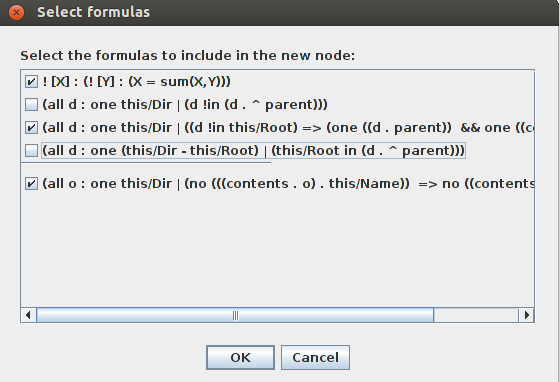
\includegraphics[width=200px]{img/select.png}
	\centering
	\caption{(Cuadro de di'alogo de proyecci'on de f'ormulas)}
        \label{seq selection}
\end{figure}

\subsubsection{Introducci'on de f'ormulas desde una fuente externa}

Esta operaci'on es una generalizaci'on de la regla de corte, que permite cargar f'ormulas desde un archivo de especificaci'on, ya sea escrito en el lenguaje \textit{Alloy} o en \textit{TPTP-FOF}. Al seleccionar las f'ormulas nuevas, se crean dos nodos nuevos que se agregan como hijos del nodo actual. Las f'ormulas a su vez se introducen como hip'otesis en uno de los secuentes y como tesis en el otro.

La operaci'on se puede ejecutar a trav'ez del men'u contextual que se muestra en la Fig. \ref{add antecedents 1}.


\begin{prooftree}
\AxiomC{$ \Gamma,\beta_1,\ldots, \beta_k \vdash \Delta $}
\AxiomC{$ \Gamma\vdash \beta_1,\ldots, \beta_k , \Delta $}
\RightLabel{(Regla de introducci'on de f'ormulas nuevas)}
\BinaryInfC{$ \Gamma \vdash \Delta $}
\end{prooftree}

con $\{\beta_1 \ldots \beta_k\}$ un conjunto de f'ormulas nuevas a introducir.

%\begin{prooftree}
%\AxiomC{$\alpha_1$,$\ldots$,$\alpha_n$}
%\UnaryInfC{$\alpha_{n+1}$,$\ldots$,$\alpha_m$}
%\end{prooftree}
%$$ \alpha_1,\ldots,\alpha_n \vdash \alpha_{n+1},\ldots,\alpha_m $$
%y un conjunto de f'ormulas nuevas $\{\beta_1 \ldots \beta_k\}$. El nuevo secuente es:
%\begin{prooftree}
%\AxiomC{$\alpha_1$,$\ldots$,$\alpha_n,\beta_1,\ldots, \beta_k$}
%\UnaryInfC{$\alpha_{n+1}$,$\ldots$,$\alpha_m$}
%\end{prooftree}
%$$ \alpha_1,\ldots,\alpha_n,\beta_1,\ldots, \beta_k \vdash \alpha_{n+1},\ldots,\alpha_m $$

'Esta operaci'on puede puede conservar o cambiar tanto la homogeneidad como la heterogeneidad del secuente inicial.

\begin{figure}
\centering
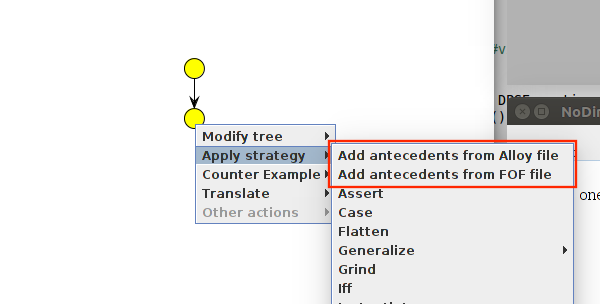
\includegraphics[width=5cm]{img/add_antecedents_1.png}	
\caption{Men'u contextual para seleccionar la fuente de las f'ormulas a introducir.}
\label{add antecedents 1}
\end{figure}


\subsubsection{Traducci'on}

Se extendi'o el concepto de traducciones para que se puedan traducir f'ormulas por separado, en lugar de traducir un secuente completo como en la versi'on anterior.
El secuente resultante contendr'a las f'ormulas del secuente analizado en el lenguaje seleccionado.

\begin{prooftree}
\AxiomC{$ \rho_{\mathcal{T}(\alpha_1)}(\alpha_1) ,\ldots, \rho_{\mathcal{T}(\alpha_n)}(\alpha_n) \vdash \rho_{\mathcal{T}(\alpha_{n+1})}(\alpha_{n+1}) ,\ldots,\rho_{\mathcal{T}(\alpha_m)}(\alpha_m) $}
\RightLabel{(Regla de traducci'on)}
\UnaryInfC{$ \alpha_1,\ldots,\alpha_n \vdash \alpha_{n+1},\ldots,\alpha_m $}
\end{prooftree}

donde $\rho_l$ es la funci'on de traducci'on al lenguaje $L$ y $\mathcal{T}:Formula\rightarrow Lenguaje$ que indica el lenguaje seleccionado para cada f'ormula del secuente original.

%$$ S: \alpha_1,\ldots,\alpha_n \vdash \alpha_{n+1},\ldots,\alpha_m $$
%\begin{prooftree}
%\AxiomC{$\alpha_1$,$\ldots$,$\alpha_n$}
%\UnaryInfC{$\alpha_{n+1}$,$\ldots$,$\alpha_m$}
%\end{prooftree}
%y una función  $\mathcal{T}:Formula\rightarrow Lenguaje$ que indica el lenguaje seleccionado para cada f'ormula del secuente $S$, el secuente resultante es:
%$$ S': \beta_1,\ldots,\beta_n \vdash \beta_{n+1},\ldots,\beta_m $$
%\begin{prooftree}
%\AxiomC{$\beta_1$,$\ldots$,$\beta_n$}
%\UnaryInfC{$\beta_{n+1}$,$\ldots$,$\beta_m$}
%\end{prooftree}


En la Fig. \ref{GUI form translation} se puede ver un cuadro de di'alogo donde el usuario puede seleccionar, para cada f'ormula, el lenguaje al que se quiere traducir.

\begin{figure}[]
	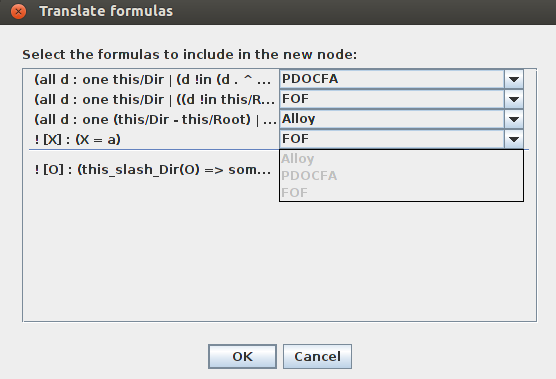
\includegraphics[width=200px]{img/translate.png}
	\centering
	\caption{Cuadro de di'alogo para la traducci'on de f'ormulas en un secuente.} \label{GUI form translation}
\end{figure}




%objetivo 3
\section{Rediseño del 'Arbol de An'alisis}

Para solucionar las limitaciones presentadas nos propusimos rediseñar el 'arbol de an'alisis.
El primer cambio que realizamos es la implementaci'on de \emph{heterogeneidad completa}.
Para lograr esto permitimos que también los secuentes sean heterogéneos, es decir, que puedan contener f'ormulas escritas en distintos lenguajes. De esta manera se consigue realizar las demostraciones con mayor flexibilidad y poder utilizar el lenguaje m'as apropiado para describir la propiedad que cada f'ormula enuncia.
La implementaci'on y los fundamentos te'oricos se explican con mayor detalle en la secci'on \hyperref[sec:heterogeneidad-verdadera]{\ref*{sec:heterogeneidad-verdadera} }.

En el 'arbol de an'alisis este cambio se refleja en la visualizaci'on de los nodos. Los nodos con secuentes heterogéneos se marcan con una \textit{H} mientras los nodos homogéneos no llevan ninguna marca.

\begin{figure}[tbh]
	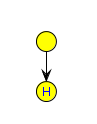
\includegraphics[width=50px]{img/hetero_homo.png}
	\centering
	\caption{El nodo con H contiene un secuente heterog'eneo. El otro nodo es homog'eneo.}
\end{figure}


\subsection{Ramas alternativas}

Para permitir documentar todas las acciones aplicadas as'i como la creaci'on de caminos de an'alisis alternativos introdujimos la noci'on de \textit{ramificaci'on alternativa}.
Las ramas alternativas representan la existencia de m'ultiples caminos en los que se subdivide el an'alisis para lograr un resultado. En la interfaz de usuario de Heterogenius este tipo de ramas se representa con lineas punteadas y su significado sem'antico es el de una disyunci'on. Se corresponde con un camino alternativo en una demostraci'on.

\begin{figure}[htb]
	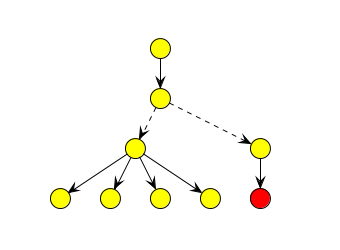
\includegraphics[width=180px]{img/ramas_alternativas_2.png}
	\centering
	\caption{La segunda rama alternativa presenta un contraejemplo. esto indica que existe un contraejemplo para el nodo del cual salen las ramas alternativas.}
        \label{alter1}
\end{figure}

Un nodo con hijos conectados por ramas alternativas se entiende que vale si \textit{\textbf{alguna}} de las ramas valen. Esto es diferente de la ramificaci'on normal (lineas continuas) que indica que el nodo padre vale si todos sus hijos valen.

Al aplicar una ramificaci'on alternativa a un nodo del 'arbol de an'alisis, el nodo es copiado y agregado como sus propios hijos. Esto nos permite trabajar sobre las copias del nodo original. Cuando es necesario tambi'en se puede agregar ramas alternativas durante un an'alisis.
 
La principal ventaja de usar caminos alternativos es la de poder documentar todo el an'alisis que se realiz'o y las decisiones tomadas, incluso las decisiones que no llevaron al cumplimiento del objetivo. Por otro lado tambi'en nos permite experimentar con diferentes formas de probar lo mismo.
En las Fig.~\ref{alter1} y \ref{alter2} se muestran ejemplos de estos usos.

\begin{figure}[bth]
	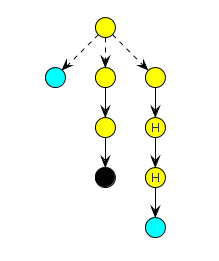
\includegraphics[width=100px]{img/ramas_alternativas.png}
	\centering
	\caption{Tres ramas alternativas: la primera y la 'ultima indican que no se encontr'o ning'un contraejemplo. La segunda rama muestra que se pudo demostrar que el secuente vale, por lo cu'al el secuente del nodo raiz tambi'en vale.}
        \label{alter2}
\end{figure}



\subsection{Nueva Clasificaci'on de Acciones}

Como se ha mencionado, el elemento principal del proceso de demostración en Heterogenius es el 'arbol de an'alisis. All'i es donde se realizan todas las acciones y es donde se refleja el camino tomado para lograr una demostraci'on exitosa. Cada nodo del 'arbol representa un secuente en alg'un lenguaje soportado por Heterogenius. Las aristas se corresponden con las acciones aplicadas a cada secuente. Dependiendo del lenguaje en el que est'e el secuente se habilitan distintas acciones, pero en general se las puede dividir en tres categor'ias:

\begin{description}
\label{clasificacion}
\item[\textbf{reglas del c'alculo de secuentes}:] son acciones que transforman un secuente en otro. Algunas pueden producir múltiples secuentes (por ejemplo la acci'on \emph{Case}) creando varias ramas que tienen que ser demostradas para lograr un resultado en el nodo raiz.

\item[\textbf{traducciones}:] traducen un secuente de un lenguaje a otro. Dependiendo de la expresividad del lenguaje esta traducci'on puede preservar completamente la semántica o sólo parcialmente.

\item[\textbf{búsquedas de contraejemplos}:] implican el uso de herramientas externas para buscar contraejemplos para intentar validar el secuente donde se aplica la acci'on. 
Dependiendo del lenguaje del secuente y del poder de la herramienta seleccionada para realizar la búsqueda, estos procesos pueden verse como análisis parciales ya que podría ser imposible agotar todo el espacio de búsqueda. En tales contextos, una búsqueda infructuosa no brinda mayor información. Por el contrario, la existencia de un contraejemplo es prueba suficiente para saber que la rama en cuestión no podrá ser cerrada.
\end{description}

Si bien esta clasificaci'on serv'ia en la versi'on anterior, debi'o ser modificada para adaptarse a la nueva funcionalidad incluida durante el desarrollo de este trabajo y permitir una mayor flexibilidad a la hora de agregar otras herramientas en el futuro.
La nueva clasificaci'on propuesta se muestra a continuaci'on.

\begin{description}
\item[\textbf{Acciones de c'alculo de secuentes}:] esta categor'ia es ls misma que en la versi'on anterior. Comprende las acciones que permiten avanzar en el an'alisis aplicando reglas del c'alculo de secuentes.

\item[\textbf{Acciones de herramientas estructurales}:] son acciones que trabajan directamente sobre la estructura del 'arbol de an'alisis. Los traductores-$\rho$ forman parte de 'este grupo, asi como las nuevas acciones introducidas: \textit{traducci'on-$\rho$ de f'ormulas} y \textit{proyecci'on de f'ormulas}.

\item[\textbf{Acciones de herramientas automáticas}:] este grupo representa a las acciones para las que se usan herramientas autom'aticas como lo son los demostradores autom'aticos de teoremas y los buscadores de contraejemplos.
\end{description}

Esta clasificaci'on se reflej'o en la arquitectura de Heterogenius y permitir'a guiar las futuras extensiones y funcionalidades adicionales que se deseen implementar.


